\IEEEpubidadjcol
\vspace{-0.6cm}
\section{Background and Motivation}
\subsection{Image Diffusion Transformer}
%
DiTs employ an encoder-based architecture, comprising Query-Key-Value (QKV) generation, multi-head attention layers, and feedforward networks (FFN). 
%
Iterative inferences of these layers incur high latency, even on datacenter-level GPUs.
%
For instance, we observe that Stable Diffusion 3 takes 18.75 seconds for generating a 1,024$\times$1,024 image on RTX-3090.

% iterative denoising process 를 통해 random noise 에서부터 점진적으로 noise 를 제거하고, 결과적으로 이미지가 만들어짐 
% SOTA image generation 모델 들은 transformer 구조로 이루어져 있음.
% encoder-based transformer 구조임 (QKV generation, attention, FFN)
% transformer 를 여러 번 추론해야 하기 때문에 연산량이 매우 많고, latency 가 매우 긺
\vspace{-0.4cm}
\subsection{Quantization for Improving Performance}
\vspace{-0.1cm}
\niparagraph{Quantization for DiT.}
Quantization is a technique that converts floating-point representations into low-precision formats, which helps reduce the memory footprint and improve the computation efficiency.
% Quantization is a well-established technique for enhancing the performance of deep neural networks. 
% By converting floating-point representations into low-precision formats, it is possible to reduce memory footprint and increase processing speed. 
% Across various quantization methods, post-training quantization (PTQ) is extensively used as it allows pretrained models to be quantized without additional training processes.
Several prior works~\cite{ptq4dit, qdit, viditq} have explored the use of quantization for DiTs.
%
These studies typically use integer (INT) quantization, applying 4-bit for weights, while retaining 8-bit for activations, which limits speedup.
% Quantization 은 DNN 의 performance 를 높이기 위한 잘 알려진 방법 중 하나임 
% floating point representation 을 low precision format 으로 바꿈으로써 memory footprint 를 줄일 수 있고, processing 속도를 높일 수 있음 
% Quantization 방식 중, post-training quantization(PTQ) 는 costly model training 없이, pretrained model 을 profiling 을 통해 quantize 할 수 있기 때문에 practically 많이 사용되는 방식이다. 
% diffusion quantization prior work 이 있다. 얘네들은 INT 쓴다. 

% Figure: BFP 설명 / MX 설명
\begin{figure}[b]
\centering
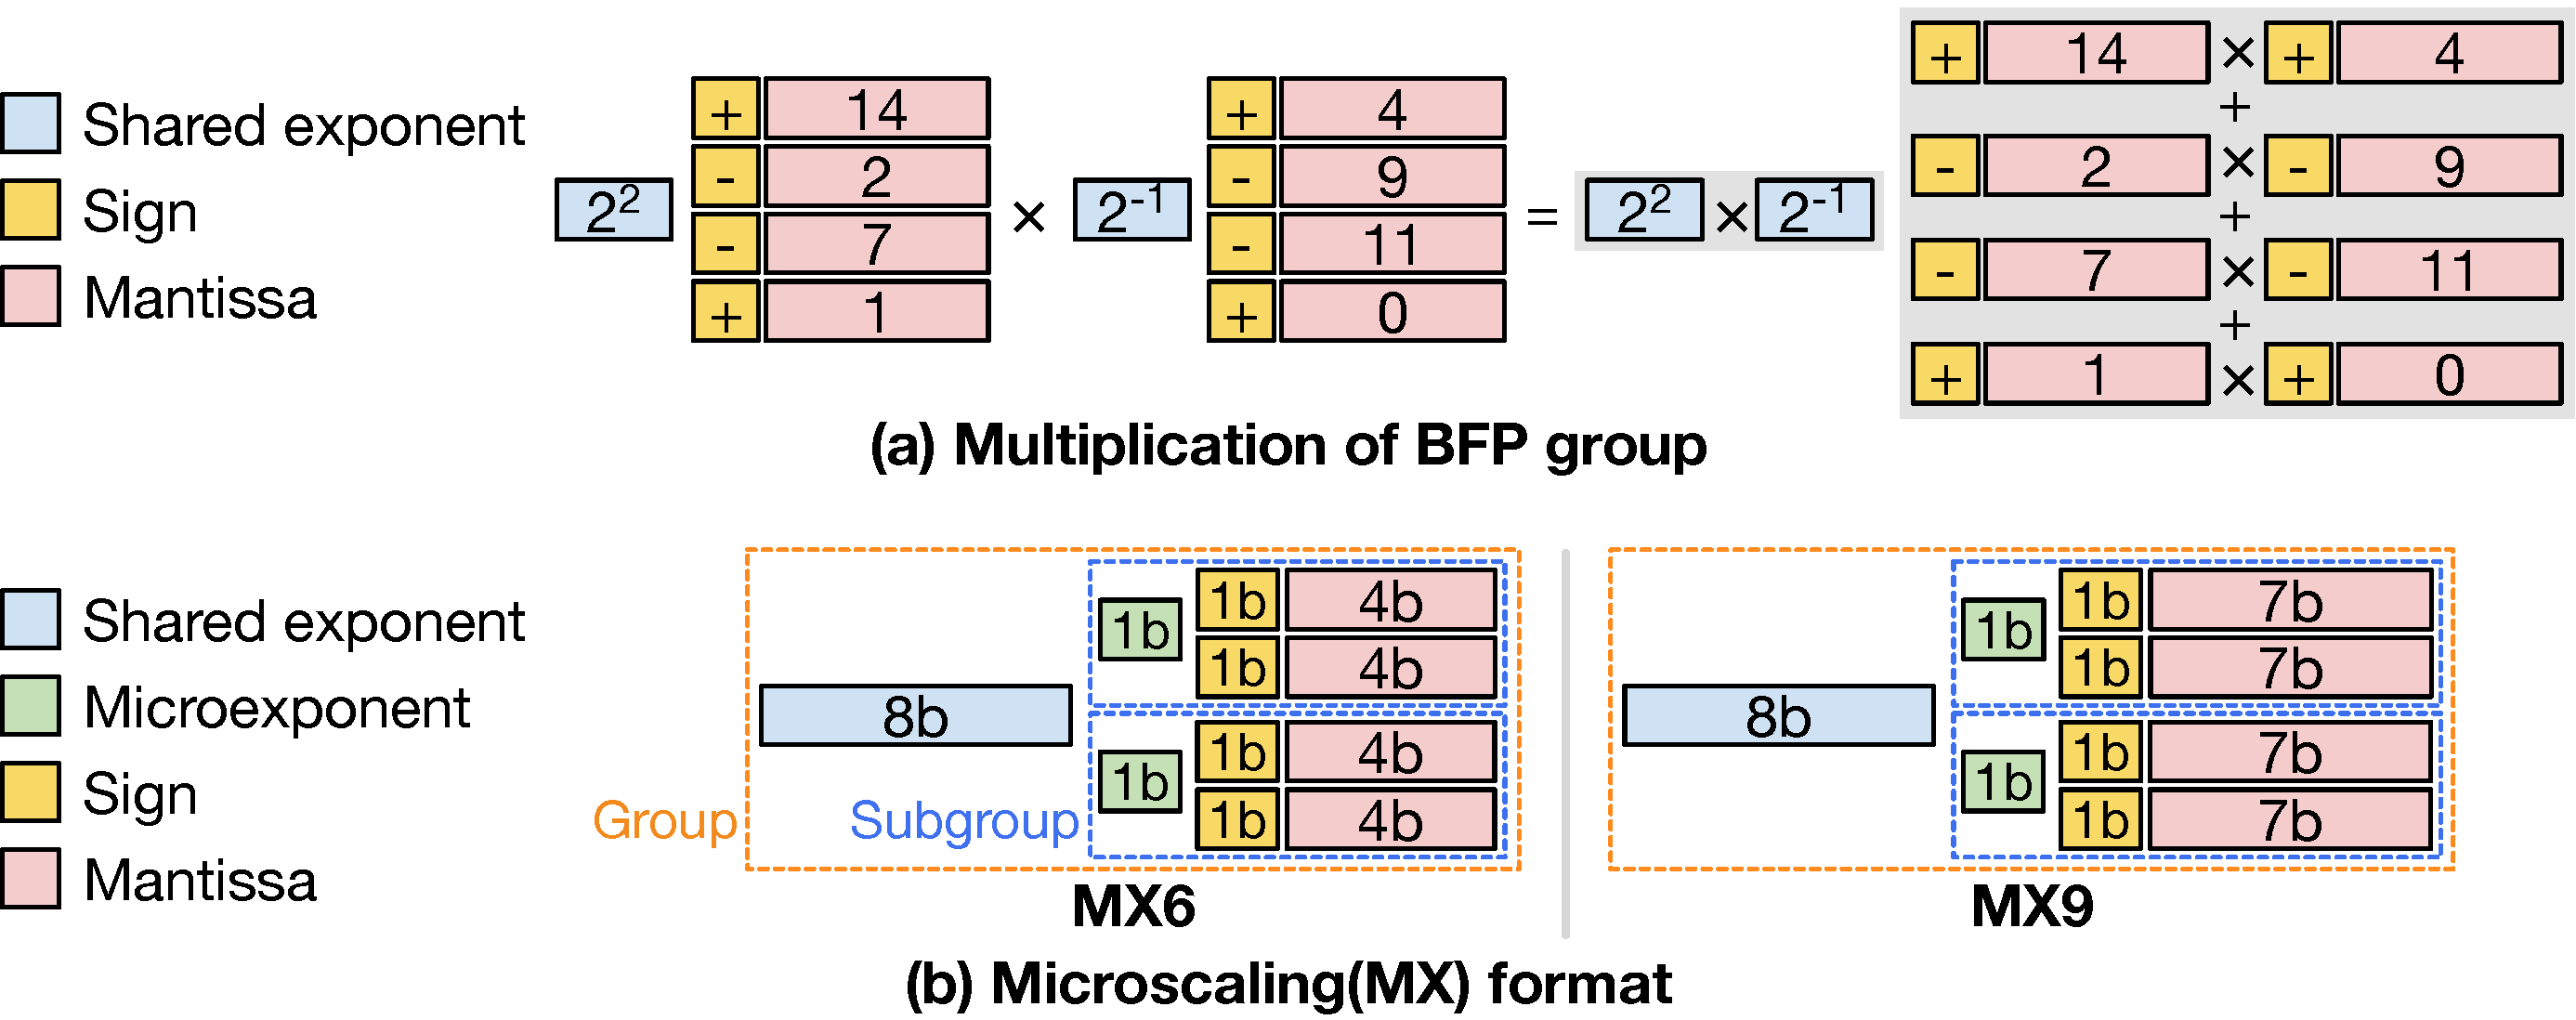
\includegraphics[width=\linewidth]{fig/bfp.pdf}
\caption{Block floating point and microscaling (MX) formats. While our design uses a group size of 16, the illustration depicts a group size of 4 for clarity.}
\label{fig:bfp}
\end{figure}

\IEEEpubidadjcol
\niparagraph{Microscaling (MX) format.}
%
Block floating point (BFP) is one of the low-precision formats that has gained attention for balancing accuracy and computational efficiency.
%
Figure~\ref{fig:bfp}(a) shows how BFP multiplication operates.
%
Unlike conventional floating point, BFP simplifies multiplication by grouping values that share an exponent.
%
Microscaling (MX) format~\cite{mx, ocp} is a variant of BFP, as shown in Figure~\ref{fig:bfp}(b).
%
MX has demonstrated potential in LLMs but has not yet been explored for DiTs.
%
This work first characterizes the challenges of applying MX to DiT-based models and then leverages these insights to develop \emph{mixed-precision} MX quantization for DiTs.
%
% MX 는 LLM 쪽에서 두각을 나타내고 있는데, diffusion transformer 에는 아직 적용된 적이 없었음. 
% 그래서 우리는 MX 를 diffusion transformer 에 사용했을 때의 문제를 characterize 해 보려고 한다. 
% 또한, diffusion transformer 에서의 특징을 이용해서 low precision MX quantization 을 해 보려고 한다. 

% 최근에는 MX 라는 놈이 떠오르고 있다. 
% MX 는 LLM 쪽에서 많이 적용되었는데, diffusion transformer 에는 적용된 예시가 없더라. 
% 우리가 그래서 처음 해 봄. 
% LLM 쪽에서 smoothquant 같은 걸 했던 노력들이 있었는데, 우리는 그 특징을 사용해서 low bit quantization 을 해 보려고 한다. 



% \IEEEpubidadjcol
\vspace{-0.3cm}
\subsection{Challenges of Applying MX formats to DiT}
\vspace{-0.15cm}
%
\niparagraph{Activation sensitivity to low precision.}
%
Table~\ref{tab:mx-degrade} presents the image quality (FID; lower is better) after applying the MX format to Stable Diffusion 3.
%
Applying MX6 to the weights while using MX9 for the activations preserves image quality comparable to FP16, whereas applying MX6 to both weights and activations causes a noticable degradation in image quality.
%
This is due to the value distribution of DiTs.
%
Figure~\ref{fig:distribution} illustrates the magnitude distribution of values in the weight and activation matrices, revealing more pronounced outliers in the activation matrix.
%
These outliers in activations significantly contribute to degradation.

%
\niparagraph{Source of quality degradation.}
%
Figure~\ref{fig:truncation} illustrates two primary ways in which large-magnitude values degrade quality.
%
First, inliers within the same group as outliers are truncated because the shared group exponent is set to the largest exponent in the group, leading to precision loss in smaller values.
%
Second, large-magnitude values experience significant quantization error when represented with a 4-bit mantissa, whereas small-magnitude values remain more precise.
%
This work proposes a mixed-precision approach to mitigate these degradations caused by large-magnitude values.
%


% \begin{table}[t]
% \centering
% \footnotesize
% \caption{Image quality after applying MX to Stable Diffusion 3}
% \label{tab:mx-degrade}
% \begin{tabular}{c|c}
% \hline
% Precision (W/A)         & FID in COCO-1k ($\downarrow$) \\
% \hline
% FP (16/16)   & 74.07 \\ 
% \hline
% MX (9/9)     & 72.98 \\ 
% \hline
% MX (6/9)     & 71.88 \\
% \hline
% MX (9/6)     & 203.37 \\
% \hline
% MX (6/6)     & 199.78 \\
% \hline
% \end{tabular}
% \end{table}


\begin{table}[t]
\centering
\footnotesize
\caption{Image quality after applying MX to Stable Diffusion 3}
\label{tab:mx-degrade}
\begin{tabular}{ccc} 
% \toprule
\hline
Method              & Precision (W/A) & FID in COCO-1k ($\downarrow$)  \\ 
% \midrule
\hline
FP                  & 16/16           & 74.07                       \\
% \midrule
\hdashline[1pt/1pt]
\multirow{4}{*}{MX} & 9/9             & 72.98                       \\
                    & 6/9             & 71.88                       \\
                    & 9/6             & 203.37                      \\
                    & 6/6             & 199.78                      \\
% \bottomrule
\hline
\end{tabular}
\end{table}


\begin{figure}[t]
\centering
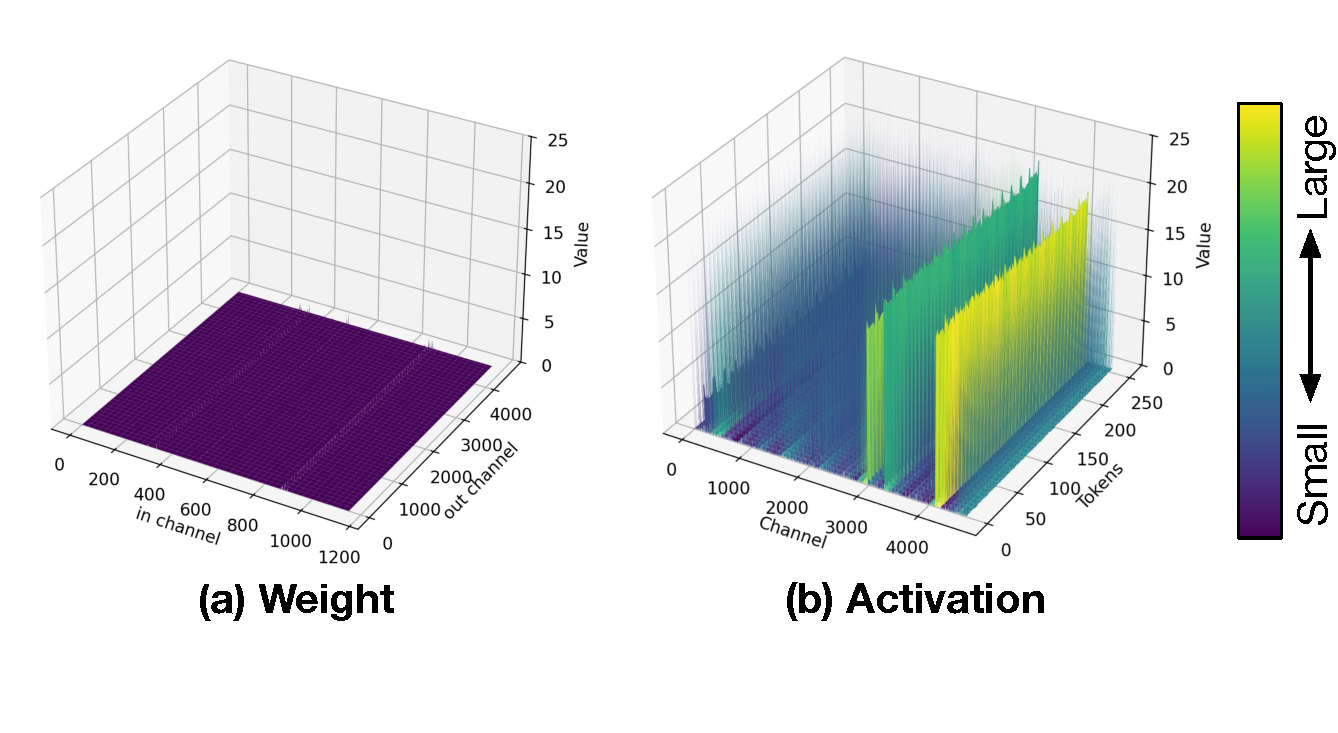
\includegraphics[width=0.8\linewidth]{fig/distribution.pdf}
\caption{Magnitude distributions of weights and activations in DiT-XL-256.}
\label{fig:distribution}
\end{figure}


\begin{figure}[t]
\centering
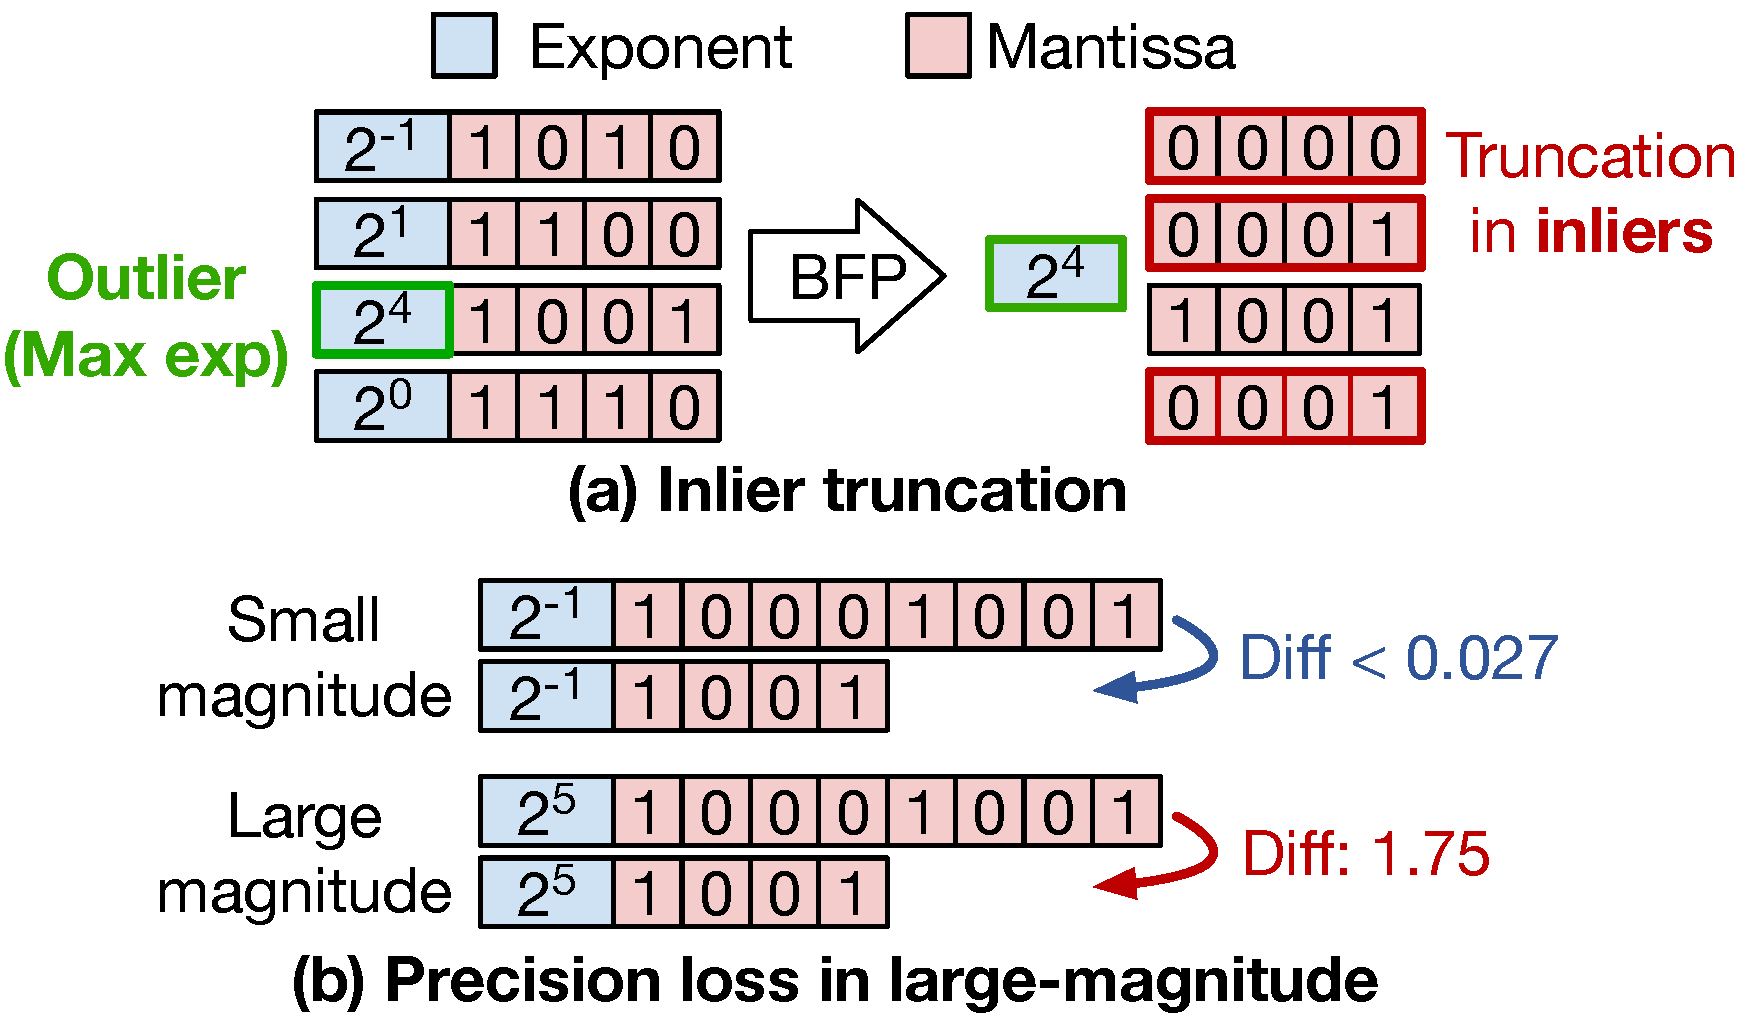
\includegraphics[width=0.75\linewidth]{fig/degradation.pdf}
\caption{Impact of large-magnitude values on MX quantization degradation.}
\label{fig:truncation}
\end{figure}


% \begin{figure}[t]
% \centering
% \subfloat[weight]{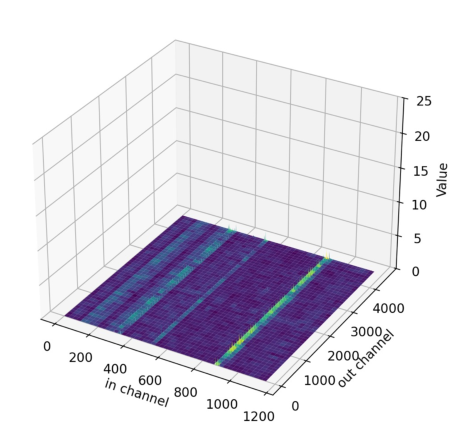
\includegraphics[width=0.4\linewidth]{fig/weight.pdf}%
% \label{fig:weight}}
% \hfil
% \subfloat[activation]{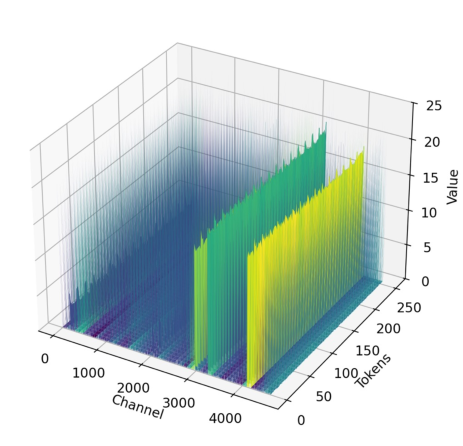
\includegraphics[width=0.4\linewidth]{fig/activation.pdf}%
% \label{fig:activation}}
% \caption{Weight and activation value magnitude visualization of DiT-XL-256. Outliers are present in specific channels and, more notably, in the activation matrix.}
% \label{fig:distribution}
% \end{figure}
